\section{Numerical simulation}%
\label{sec:numericalsetup}
In order to extract the quantum properties of the discretized system (equations \ref{eqn:energy} and \ref{eqn:matelem}) and recover the continuum results (equations \ref{eqn:phys1} and \ref{eqn:phys2}) we have to compute the correlators $\ct$, defined as the $N-$dimensional integral in equation
\ref{eqn:integral}.
We proceed numerically, via the importance sampling Monte Carlo method, using the Metropolis
algorithm to design an ergodic Markov chain with asymptotic probability distribution $\nicefrac{e^{-S}}{Z}$.
The chain will be used to extract the random variables needed for the integration, which are physically equivalent to considering
different Feynman paths.

In this section we discuss the Metropolis algorithm and the subsequent Markov chain in greater detail.
The data shown, unless explicitely specified, have been computed using the following lattice parameters.
\begin{table}[ht]
\centering
\begin{tabularx}{0.6\linewidth}{cccc}
\hline
\multicolumn{4}{c}{Parameters} \\ \hline
$N$              & $256$  & $m$              & $1$      \\
$a$              & $0.25$ & $\w$             & $1$      \\
$N_{sweep}$      & $1e6$   & $\Delta$ & $1$ \\ \hline
\end{tabularx}
\caption{\label{tab:A3}Parameters used for the analysis shown in the next sections.}
\end{table}
\subsection{Monte Carlo method}%
\label{subsec:montecarlo}
As highlighted in the previous section, the initial goal of the simulation is the numerical evaluation
of the integral in equation \ref{eqn:integral}.
The random variables needed for the integration are the Feynman paths\\ $E_{J}\equiv\{x_{0},\dots,x_{N-1}\}_{J}$.

To ensure that each new configuration is extracted following the right probability distribution
$\nicefrac{e^{-S}}{Z}$, we choose to work with an ergodic Markov chain.
Indeed, an ergodic Markov chain with probability transition matrix $P_{JK}$ is guaranteed to have
an asymptotic distribution $\pi_{J}$ whose form does not depend on the starting configuration; thus, we just need to design an ergodic Markov chain such that $\pi_{J}=\nicefrac{e^{-s}}{Z}$.



A sufficient condition for a Markov chain to be ergodic is for it to obey the detailed balance $\pi_{J}P_{JK}=\pi_{K}P_{KJ}$ and a sufficient condition for a Markov chain to satisfy the detailed balance is to be generated by the Metropolis algorithm. Therefore, it is enough for us to implement the Metropolis algorithm to eventually generate suitable configurations -- \textit{i.e.} suitable Feynman paths.

The Metropolis Monte Carlo algorithm is composed of two steps

\begin{enumerate}
  \item \textbf{Proposal:} given an initial state $E_{J}$, a state $E_{K}$ with transition probability $Q_{JK}$ satisfying
        the microreversibility condition\footnote{$Q_{JK}=Q_{KJ}$} is proposed;
  \item \textbf{Accept/Reject:} to generate events with asymptotic probability distribution $\pi_{J} = \nicefrac{R_{J}}{\sum_{J}R_{J}}$\footnote{Note that this has the same form of $\nicefrac{e^{-S}}{Z}$.},
        the new configuration is accepted with probability $1$ if $R_{K}\ge R_{J}$ and with probability
        $\nicefrac{R_K}{R_J}$ otherwise. Thus, we construct a transition probability matrix
      \begin{align}
          P_{JK}=
          \begin{cases}
            Q_{JK} \text{ if } R_{K}\ge R_{J}\\
            Q_{JK}\dfrac{R_{K}}{R_{J}} \text{ if } R_{K}<R_{J}
          \end{cases}.
        \end{align}
\end{enumerate}
If a new configuration is rejected, the algorithm \\restarts from $E_{J}$ and a new proposal is made.

In our implementation the asymptotic distribution is $\nicefrac{e ^{-S}}{Z}$, so a new proposal $E_{K}$ is certainly accepted if the action decreases\footnote{$\Delta S = S[E_{K}]-S[E_{J}] < 0$.}
and accepted with probability $e ^{-\left(S[E_{K}]-S[E_{J}]\right)}$ if the action increases.
Configurations that correspond to larger actions are still allowed, but they are at a disadvantage compared to those that lead to smaller actions.
The algorithm makes a new proposal for each coordinate $x_i$, one at a time, of the starting configuration. That is
\begin{align}
  &E_{K} = \{x_{0}, \dots, x_{i}, \dots, x_{N-1}\} \mapsto \notag \\
  &E_{K+1}=\{x_{0}',\dots,x_{i},\dots x_{N-1}\} \mapsto \notag \\
  &\vdots \notag \\
  &E_{K+N}=\{x_{0}', \dots,x_{i}', \dots, x_{N-1}'\}.
\end{align}
Once every coordinate has undergone the accept/reject phase we
say that a \textit{sweep} has happened and \textit{Markovian time} increases by one unit (figure \ref{fig:sweep}).
\begin{figure}[ht]
  \centering
  \ctikzfig{sweep}
  \caption{\label{fig:sweep}The elementary step of the Markov chain consists of the (potential) update of one coordinate, after the elementary step has happened for every coordinate a sweep is completed. The sweep index
    is called \textit{Markovian time}. After a sufficiently large number of sweeps, the chain
    is said to be thermalized and each new random $x_{i}$ will be extracted following $\nicefrac{e ^{-S}}{Z}$. Physically, a new sweep is a new Feynman path.}
\end{figure}


The proposal for an updated coordinate  $x_{i}' \mapsfrom x_{i}$ is chosen in the closed interval $[x_{i} - \Delta, x_{i} +\Delta]$ ($\Delta$ is
a positive, real algorithm parameter that does not impact the physics)
and it depends on a random number $r_{1}$, generated with uniform distribution
between $0$ and $1$\footnote{As $r_{1}$ is chosen with a flat distribution microreversibility is guaranted -- \textit{i.e.} the transition $x_{i}\mapsto x_{i}' $ is equiprobable to the transition $x_{i}'\mapsto x_{i}$.}
\begin{align}
  \label{eqn:proposal}
  x_{i}' = x_{i}+ 2\Delta \left(r_{1} - \frac{1}{2}\right).
\end{align}
The accept/reject phase of the algorithm is implemented with a second random number $r_{2}$, also generated with uniform distribution
between $0$ and $1$
\begin{align}
  \begin{cases}
    \text{if } e ^{-\Delta S} \ge r_{2} \text{ accept } x_{i}'  &\implies x_{i} \mapsto x_{i}' \neq x_{i} \\
    \text{if }e ^{-\Delta S} < r_{2} \text{ reject } x_{i}' &\implies x_{i} \mapsto x_{i}' \equiv x_{i}
  \end{cases}.
\end{align}
Since the chain only tries to update one coordinate at a time, if we call the coordinate shift $\delta x_{i}$, the
corresponding variation of the action is
\begin{align}
  \Delta S = \frac{m}{2a}\delta x_{i}\qty[\left(2+a ^2\w ^2\right)\left(2x_{i}+\delta x_{i}\right) - 2(x_{i+1}+x_{{i-1}})].
\end{align}
Now the discussion of the experiment can begin, starting from the thermalization of the chain.

\subsection{Thermalization of the chain}%
\label{subsec:thermalization}
Before the chain reaches its asymptotic probability distribution we need to let it evolve for a number of sweeps. Figure \ref{fig:therminit} shows that
the thermalization value is reached independently of the initialization values of $E_{J}$ for a given lattice, which we initalized in four
ways:
\begin{enumerate}
  \item with random numbers between $-1$ and $1$;
  \item  with random numbers between $-5$ and $5$;
  \item setting $x_{i}=0\ \forall i$ (cold initialization);
  \item setting $x_{i}=10\ \forall i$ (hot initialization).
\end{enumerate}
\begin{figure}[htp]
  \centering
  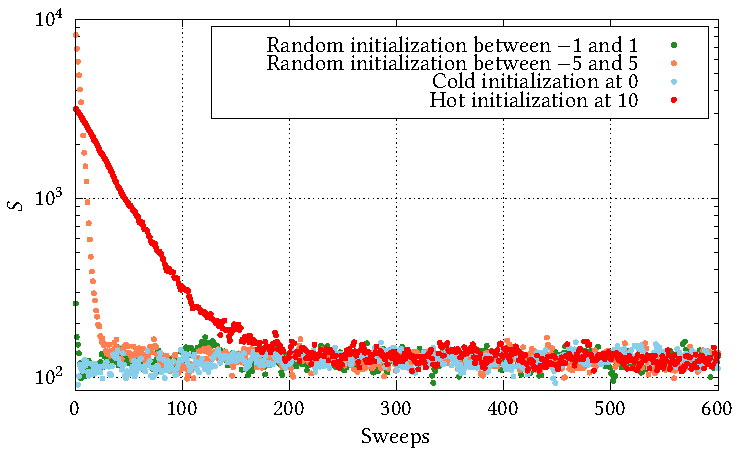
\includegraphics[width=\linewidth]{therminit}
  \caption{\label{fig:therminit} Thermalization of different Markov chains. Regardless of their initialization, they eventually start oscillating around an equilibrium value.}
\end{figure}
It is worth noting that while the thermalization value is the same, the speed is different. The \textit{colder} initialized chains take $\sim 30,50$ sweeps to thermalize, while the \textit{hot} chain needs around $\sim 200$. As a safety measure, while a colder initialization
was generally preferred,
due to the low computational costs of sweeping we decided to let each chain thermalize for $N_{therm}=1000$ sweeps\footnote{This proved to be more than enough for every lattice we considered.} throughout the whole simulation.

As we will see in subsection \ref{subsec:delta}, the width of the interval used to extract the coordinate update proposals $x_{i}'$ has an effect on the thermalization speed.

Once the chain is thermalized, it is sensible to compute the correlators.

\subsection{Improved observables}%
\label{subsec:improved}
The integrals we are interested in are of the form
\begin{align}
  \label{eqn:form}
  \ev{O(x_{l})O(x_{k})} = \frac{1}{Z(T,a)}\int \prod_{i=0}^{N-1}\dd{x_{i}}e^{-S}O(x_{l})O({x_{k}}),
\end{align}
whose best estimate is
\begin{align}
  \label{eqn:Omean}
  \overline{O(x_{l})O(x_{k})} = \frac{1}{N_{config}}\sum_{n=1}^{N_{config}}O(x_{l})_{n}O(x_{k})_{n}
\end{align}
in the limit of large $N_{config}$. Clearly, the value of the integral is
\begin{align}
   \ev{O(x_{l})O(x_{k})} = \lim_{N_{config}\to\infty}  \overline{O(x_{l})O(x_{k})}.
\end{align}

Furthermore, we can exploit the path integral's translational invariance to define improved observables with
smaller error. For each configuration we define
\begin{align}
  \label{eqn:Oimproved}
  O(\t)_{n} = \frac{1}{N}\sum_{i=0}^{N-1}O(x_{l+i})_{n}O(x_{k+i})_{n}
\end{align}
so that we identify $\overline{O(\t)}=\overline{O(x_{l})O(x_{k})}$ and find an improved version of the
observable \ref{eqn:Omean} as
\begin{align}
  \overline{O(\t)} = \frac{1}{N_{config}}\sum_{n=1}^{N_{config}}O(\t)_{n}.
\end{align}

Thus, the best estimate of the integral \ref{eqn:integral} is
\begin{align}
  \overline{\ct} = \ev{x_{l}x_{k}} = \frac{1}{N_{sweep}}\sum_{n=1}^{Nsweep}\ct_{n},
\end{align}
where the improved observables are, at fixed physical time $\t$ and for each Feynman path,
\begin{align}
  \ct_{n} = \frac{1}{N}\sum_{i=0}^{N-1}\qty[x_{i}x_{i+\t}]_{n}
\end{align}
and $n$ labels a thermalized sweep of the Markov chain.


\subsection{Autocorrelation and binning}
\label{subsec:autocorrelation}
At this point we are confronted with a problem. The best estimate of the correlator is an average over the number of thermalized
configurations, but each \textit{next} configuration is generated, site by site, from the \textit{previous}. In other words, the configurations corresponding to subsequent
sweeps are not independent: the observables $\ct_{n}$ are correlated in Markovian time $n$.
As a consequence, in the limit $N_{sweep}\to\infty$, the variance of our numerical computation is
\begin{align}
\sigma ^2\qty[\overline\ct] = \frac{\sigma ^2\qty[\ct]}{N_{sweep}}\qty{1 + 2\sum_{n=1}^{\infty}\frac{\Gamma_{\t}(n)}{\Gamma_{\t}(0)}}
\end{align}
where $\Gamma_{\t}(n) \equiv \ev{\ct_{m} \ct_{m+n}}_{m}-\overline{\ct}^2$ is the autocorrelation function at (Markovian) time $n$\footnote{It is worth noting that $\Gamma_{\t}(0) = \sigma ^2[\ct]$}.
The ratio $\nicefrac{\Gamma_{\t}(n)}{\Gamma_{\t}(0)}$ is a measure of the correlation between two observables $\ct_{m}$ that are $n$ sweeps apart\footnote{$n$ is also known as \textit{lag}.}. Indeed, if the ratio was $0$ we would recover the variance on the mean of uncorrelated measures that we would expect.

For a Markov chain,
\begin{align}
  \label{eqn:autoratio}
  \frac{\Gamma_{\t}(n)}{\Gamma_{\t}(0)} \sim \exp\qty(-\frac{n}{\tau});
\end{align}
we call $\tau$ the \textit{autocorrelation time} and note that after $\sim 4,5 \tau$ sweeps the correlation between two observables becomes
negligible.
\begin{figure}[ht]
  \centering
  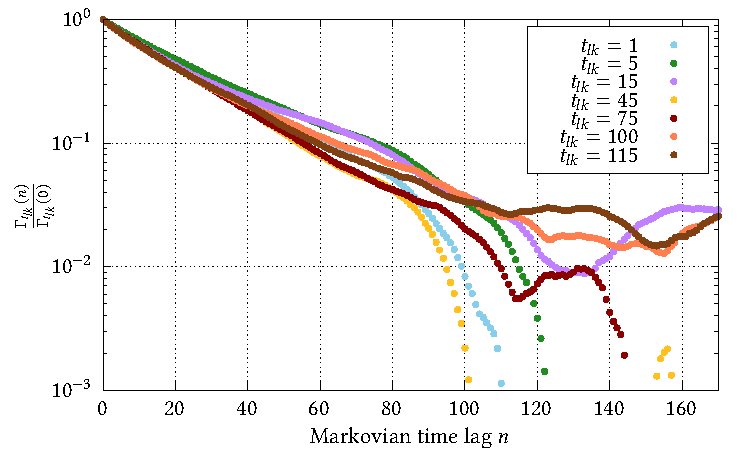
\includegraphics[width=\linewidth]{gamma.pdf}
  \caption{\label{fig:gammat} Autocorrelation  as a function of Markovian lag for observables at different fixed physical times. Its value decreases exponentially with $n$ -- $y$ axis is in $\log$ scale -- until it starts oscillating. Observables corresponding to larger physical times (equivalent to the distance of the sites on the lattice) need more sweeps to
  decorrelate.}
\end{figure}
Therefore, it is possible to decorrelate the measures through a binning procedure, in order to minimize the impact of consequent Feynman paths.
The value of $\tau$ can be determined from an exponential fit of ratio \ref{eqn:autoratio} and used to group
$D_{bin}\sim 10,100\tau$ observables together in a single bin, of which we take the average value.
As a consequence, we will now work with $N_{bin}=\nicefrac{N_{sweep}}{D_{bin}}$ decorrelated observables
\begin{align}
  \label{eqn:binned}
  \ct_{n}= \frac{1}{D_{bin}}\sum_{j=1}^{D_{bin}}\ct_{j}; \, n = 1, \dots, N_{bin}
\end{align}
on which we can apply the \textit{usual} statistical analysis over $N_{bin}$ Feynman paths, thus obtaining the best estimation of the correlator \ref{eqn:integral} as
\begin{align}
  \label{eqn:bestestim}
  \ct = \frac{1}{N_{bin}}\sum_{n=1}^{N_{bin}}\ct_{n},
\end{align}
with variance\footnote{The binning procedure on $x^{2}$ happened \textit{after} the coordinates were squared.}
\begin{align}
  \label{eqn:bestvariance}
  \sigma^{2}\qty[\ct] = \frac{1}{N_{bin}}\qty[\ev{x_{l,binned}^{2}x_{k,binned}^{2}}-\ct^{2}].
\end{align}
\begin{figure}[h]
  \centering
  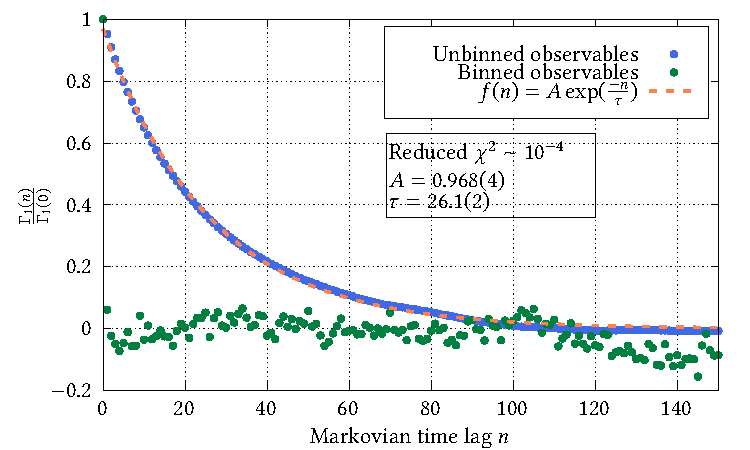
\includegraphics[width=\linewidth]{binvsnot}
  \caption{\label{fig:binvsnot}Autocorrelation for binned and unbinned correlators; the exponential fit has been done with Gnuplot. The value of $\tau=26$ was then used to determine the bin width
    $D_{bin}=500$. The binned observables, shown here in green,
  are decorrelated from the start.}
\end{figure}
\\
In figure \ref{fig:binvsnot} we show the autocorrelation for both the unbinned and the binned correlator at $\t = 1$. It takes
$\tau \sim 26$ sweeps for the unbinned observables' autocorrelation to decrease to $\nicefrac{1}{e}$, therefore we set $D_{bin}=500$. As expected,
the binned observables among different sweeps are not correlated from the start.



\subsection{The $\Delta$ parameter}%
\label{subsec:delta}
Now we are ready to investigate the effects of the different choices of the algorithm parameter $\Delta$ on the thermalization speed and autocorrelation time of the chain.
The first concept we need to introduce is the acceptance.

The proposal for an updated coordinate (equation \ref{eqn:proposal}) selects an $x_{i}'$ inside a closed interval of center
$x_{i}$ and width $\Delta$: it is reasonable that such parameter influences the efficiency of the Metropolis
algorithm. We define \textit{acceptance rate} or simply \textit{acceptance} the frequency of a new proposal getting accepted.

\begin{figure}[h!]
  \centering
 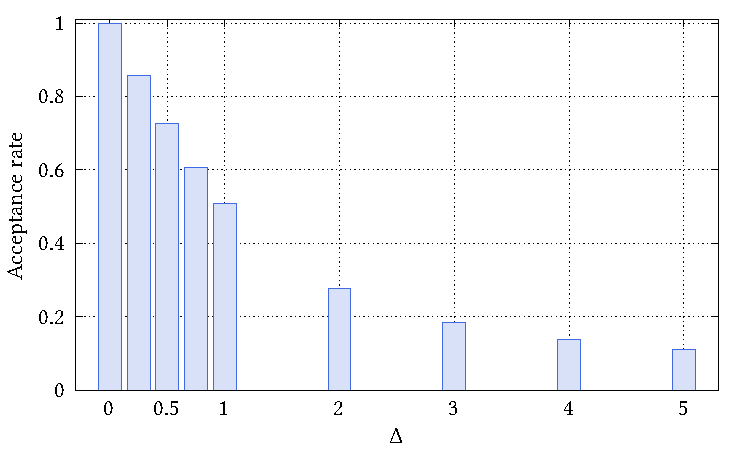
\includegraphics[width=\linewidth]{accettanza}
  \caption{\label{fig:acceptance} Acceptance rate plotted against the value of $\Delta$. Acceptance decreases for larger $\Delta$ values. }
\end{figure}

The higher the acceptance, the more likely it is that a new proposal is accepted, which is desirable from a computational
cost standpoint since it implies less \textit{void} iterations of the algorithm. On the other hand, the purpose of the Metropolis algorithm
is to iteratively refine the transition probability of a Markov chain, therefore we would like a somewhat strict selection.
Figure \ref{fig:acceptance} gives some insight on the acceptance rate for different values of $\Delta$.

The limit case with $\Delta = 0$, $\text{acceptance}=1$, is a good example of the concept above: if $\Delta = 0$, every sweep would be an exact copy of the previous
so the chain will never reach the desired thermalization value.

\begin{figure}[ht]
  \centering
  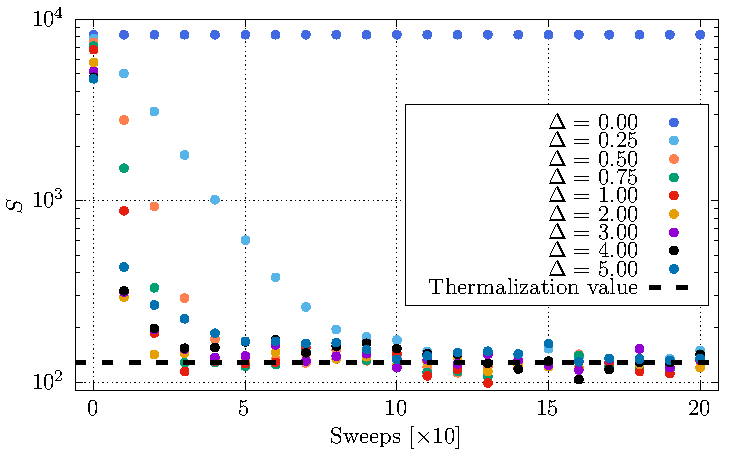
\includegraphics[width=\linewidth]{thermdelta}
  \caption{\label{fig:thermdelta}Thermalization speed for different values of $\Delta$. The action is plotted once every $10$ sweeps. If $\Delta \neq 0$, the thermalization value
  is reached with variable speed: the sweet spot seems to be around $1\le \Delta \le 3$.}
\end{figure}

Figure \ref{fig:thermdelta} shows the values of the action as a function of Markovian time, plotted once every $10$ sweeps, for different values
of $\Delta$. The thermalization time decreases up to $\Delta = 3$ and then it starts slowly growing again.

Since the composition of each configuration heavily depends on $\Delta$,
the parameter also influences the autocorrelation time $\tau_{int}$.
This dependence is analyzed in figure \ref{fig:taudelta}.
\begin{figure}[h!]
  \centering
  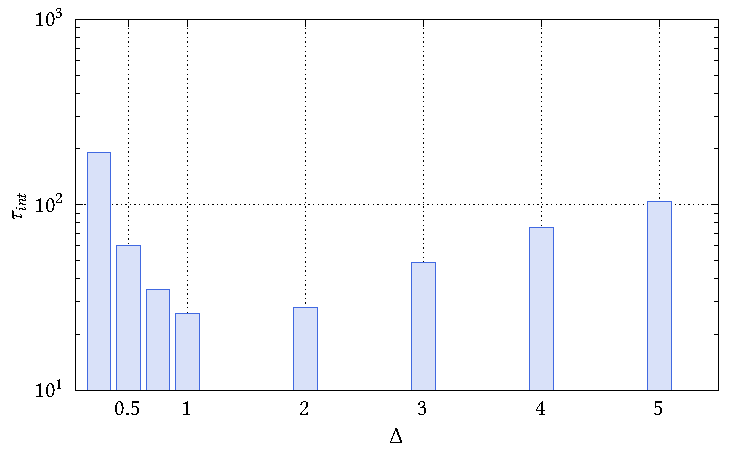
\includegraphics[width=\linewidth]{tau}
  \caption{\label{fig:taudelta}Interaction time in $\log$ scale for different values of $\Delta$. $\Delta = 0$ is not considered as every
  sweep simply copies the previous.}
\end{figure}

The interaction time decreases from $\Delta = 0.25$ to $\Delta = 1$, where it reaches its minimum, then starts growing again: this is
the parameter we decided to prioritize. Autocorrelation time is used to determine the dimension of each bin and, as a consequence, the number of
of bins for a fixed number of sweeps. In order to maximize the number of bins, we kept $\Delta = 1$ for the entire simulation.

